\section{Introduction}

The problem at hand is to investigate the properties of the ground state of a hardcore-bosonic wheel with different number of lattice sites $L$ on the ring (\autoref{fig:wheel}) using exact diagonalisation (ED) methods. 

\begin{wrapfigure}{r}{0.4\textwidth}
    \centering
    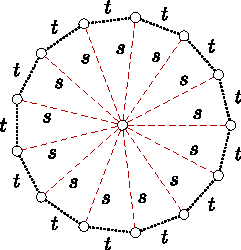
\includegraphics[width=4cm]{graphics/wheel.pdf}
    \caption{Wheel geometry with hopping amplitudes on the ring ($t$) and from the ring to the center ($s$). Illustration from the exercise sheet.}
    \label{fig:wheel}
    \vspace{-1cm}
\end{wrapfigure}

In this problem, two ways to find the ground state (energies) were proposed:
\begin{enumerate}[label=(\roman*)]
    \item The ED of a $(L+1)\times(L+1)$ matrix in the operator-valued vector basis, and
    \item The ED of a $2^{L+1}\times2^{L+1}$ matrix represented in the occupational (Fock) state basis of the tensor-product Hilbert space. 
\end{enumerate}

An immediate consequence that one notices is that the number of eigenvalues obtained for (i) would be significantly less than that from (ii) simply due to the size of the matrix. The discussion of the comparison between these two methods will be carried out in \autoref{sec:c}.

Before we go into the individual problems, we first describe the general structure of the code. The problem-specific implementation in the code shall then be described in the discussion of the problem itself. The programming language of choice was Python. Certain code segments have also been parallelised with \texttt{mpi4py}\footnote{\url{https://mpi4py.readthedocs.io/en/stable/}}, which uses the Message Passing Interface (MPI) under the hood to allow parallelisation across different computing nodes. Unfortunately, the code does not run properly on the cluster for \texttt{nstasks} $> 8$. This problem will be described further under \autoref{sec:parallelisation}. 

The personal desktop PC ultimately used for the generation of this data ran on a 8-core, 16-thread Ryzen 7 5800X, which allowed us to run the calculations with \texttt{nstasks} $= 16$ at higher processor speed ($4.5$ GHz). In the end, the data used for the graphs in this report took approximately 6 hours to generate, before the data was processed and plotted.

